\section{The Compact Muon Solenoid}

The Compact Muon Solenoid (CMS) detector is designed to provide efficient identification and 
measurement of photons, electrons, muons, taus and hadronic showers over a wide range of 
transverse momentum and direction.
CMS is divided into sub-detector systems, as can be seen in Figure \ref{fig:cms_complete}
which perform complementary roles.
The central feature of the CMS apparatus is a superconducting solenoid of 6\unit{m} internal diameter. Within the superconducting solenoid volume are a silicon pixel and strip tracker, a lead tungstate crystal electromagnetic calorimeter (ECAL), and a brass/scintillator hadron calorimeter (HCAL). Muons are measured in gas-ionization detectors embedded in the steel return yoke outside the solenoid. Extensive forward calorimetry complements the coverage provided by the barrel and endcap detectors. 
\begin{figure}[htbp]
\centering
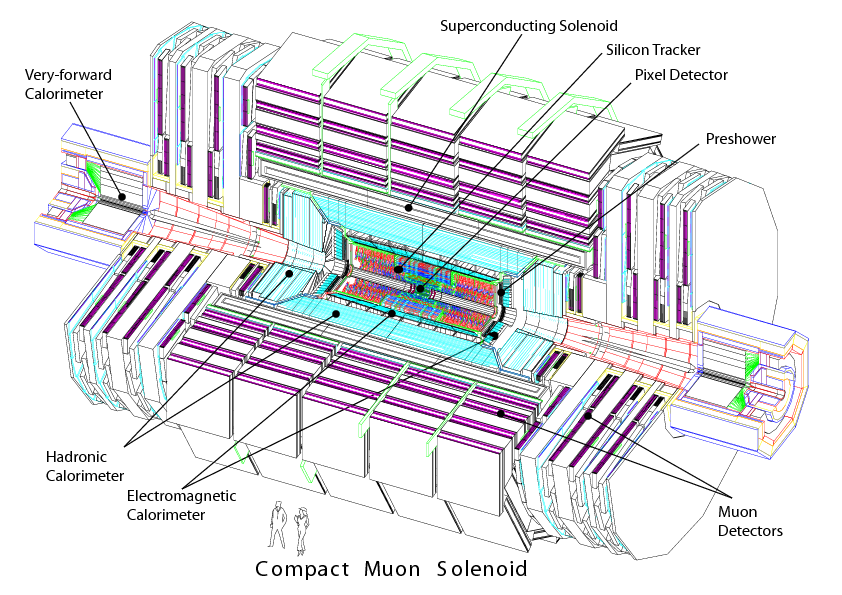
\includegraphics[width=0.9\textwidth]{plots/intro/cms_complete.png}
\caption{The Compact Muon Solenoid detector.\label{fig:cms_complete}}
\end{figure}

A more detailed description of the CMS detector can be found in Ref.~\cite{Chatrchyan:2008zzk}.  
The following sections describe in more detail the specific features of the CMS detector
that are crucial in the search for long-lived neutral particles decaying to jets, namely: the
tracking system, the particle-flow reconstruction and the jet reconstruction algorithm.

\subsection{Tracking system}

The tracker, the innermost detector system of the CMS detector, has a length
of 5.8 m and a
diameter of 2.5 m. It is immersed in a coaxial magnetic field of 3.8 T
provided by the CMS solenoid. A schematic drawing of the CMS tracker is shown in
Fig. 1. It comprises a silicon pixel detector with 3 barrel layers at radii
between 4.4 cm and 10.2 cm and a silicon strip tracker with 10 barrel
detection layers extending outwards to a radius of 1.1 m. Each system is
completed by endcaps which consist of 2 disks in the pixel detector and 3
plus 9 disks in the strip tracker on each side of the barrel, extending
the acceptance of the tracker up to a pseudorapidity of $|\eta| < 2.5$.
\begin{figure}[!h]
\centering
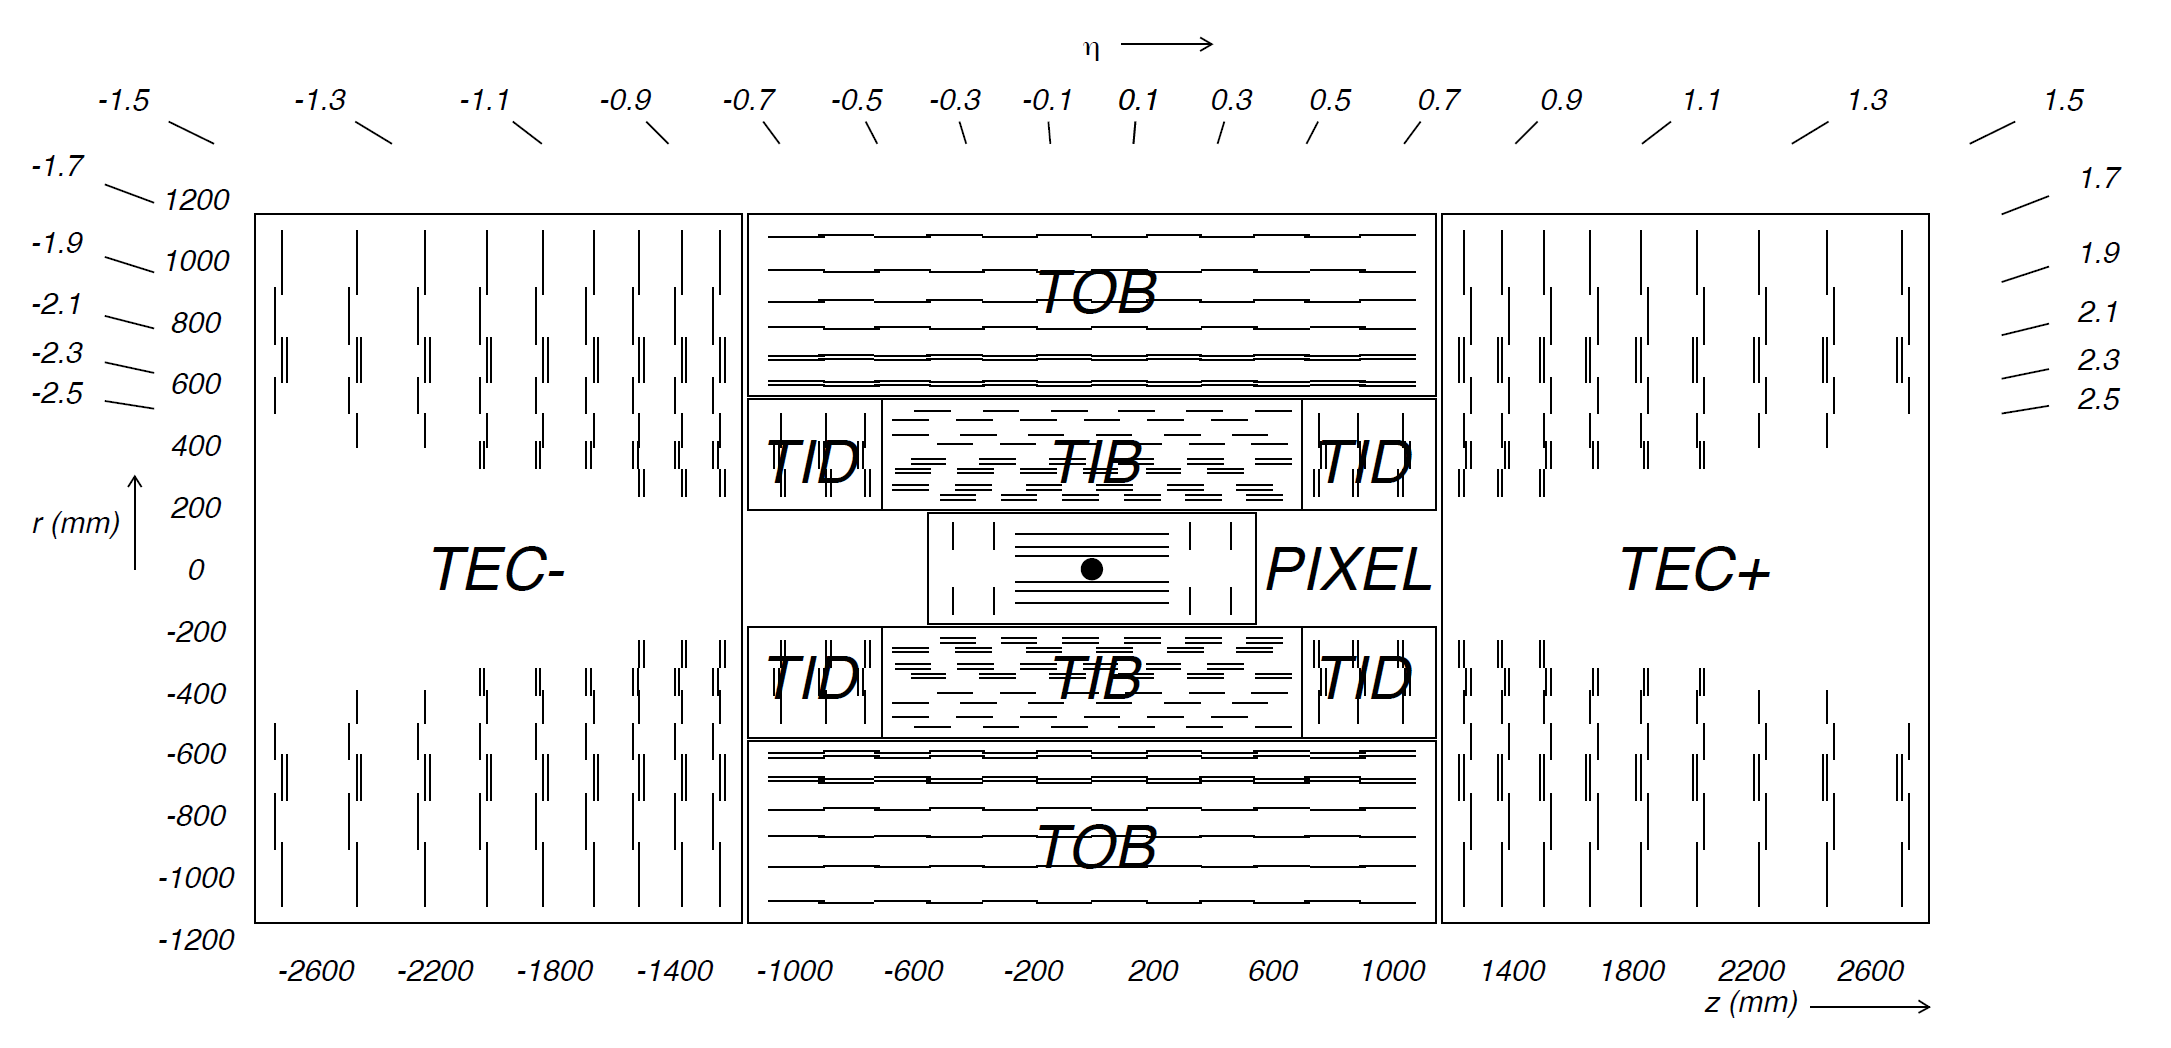
\includegraphics[width=0.99\textwidth]{plots/intro/tracker.png}
\caption{Schematic cross section through the CMS tracker. Each line represents a
detector module. Double lines indicate back-to-back modules which deliver stereo
hits.}
\end{figure}

The track reconstruction sequence is divided into 5 logical parts:
\begin{itemize}
\item \textbf{Local reconstruction} consists of clustering into \textit{hits}
the strip and pixel signals produced by charged particles on the silicon
detectors of the tracking system. The positions of the hits are estimated along
with the corresponding uncertainties;
\item \textbf{Seed generation} provides initial track-candidates for the full
track reconstruction. A seed defines initial trajectory parameters and errors;
\item \textbf{Pattern recognition} step is based on a global Kalman filter and
is responsible for finding the track-candidates that correspond to charged
particles of interest. The trajectory parameters are updated whenever a \textit{hit} is found
along the trajectory. Because the trajectories are build in parallel and allowed to share position
measurements, this part is also responsible for
cleaning the track-candidates collection by removing duplicates;
\item \textbf{Final Track fit} module estimates the final parameters of the trajectories
with ultimate precision;
\item \textbf{Track selection} rejects fake tracks by requiring that the final
tracks match a minimum set of quality criteria.
\end{itemize}

To improve the track finding efficiency, the above reconstruction procedure is
performed in six iterations. After every iteration, the hits
used for the best quality tracks (\textit{highPurity} tracks) are
locked and removed from the pool of hits available for the next iterations.
The iterations differ from each other mainly in how they
seed the tracks.
 The $0^{th}$ iteration uses pixel-triplet seeds (formed from
hits in 3 pixel layers), while the $1^{st}$ iteration uses pixel-pair seeding
(formed from hits in any 2 pixel layers), allowing it to recover tracks with
missing pixel hits due to inefficiency or acceptance. These two iterations
suffice to reconstruct the vast majority of moderately high $p_T$ tracks ($>$1GeV)
originating from the production vertex. The $2^{nd}$ and $3^{rd}$ iterations
also use pixel seeding, but since many of the Tracker hits have already been
locked by the time they run, they can use a very low $p_T$ cut or a rather
loose vertex constraint, respectively. Finally, the $4^{th}$ and $5^{th}$
iterations seed the tracks in the Strip Tracker double-layers, which provide 3D
hits by combining information from mono and stereo hits. This allows them to
find particles produced even outside the volume of the Pixel Tracker. The procedure has been optimized for using as
many tracker hits as possible while keeping the rate of fake tracks negligible.

The CMS tracker provides an impact parameter resolution of ${\sim}15\mum$ and a transverse momentum (\pt) resolution of about 1.5\% for 100\GeV particles. 
The track reconstruction algorithms are able to reconstruct displaced tracks with transverse impact
parameters up to ${\approx}30$\,cm from particles decaying up to ${\approx}60$\,cm from the beam line.  The
performance of the track reconstruction algorithms has been studied with data
\cite{Khachatryan:2010pw}. 
The silicon
tracker is also used to reconstruct the primary vertices positions with a
precision of ${\sim}20$~\mum in each dimension.

\subsection{Particle-Flow (PF) reconstruction}

The global event reconstruction (also called particle-flow event reconstruction~\cite{CMS-PAS-PFT-09-001,CMS-PAS-PFT-10-001}) is designed to reconstruct and identify each particle in the event using an optimized combination of all subdetector information.
Figure \ref{fig:cmsslice} presents schematically how various types of particles are reconstructed
with the CMS detector.

\begin{figure}[htbp]
\centering
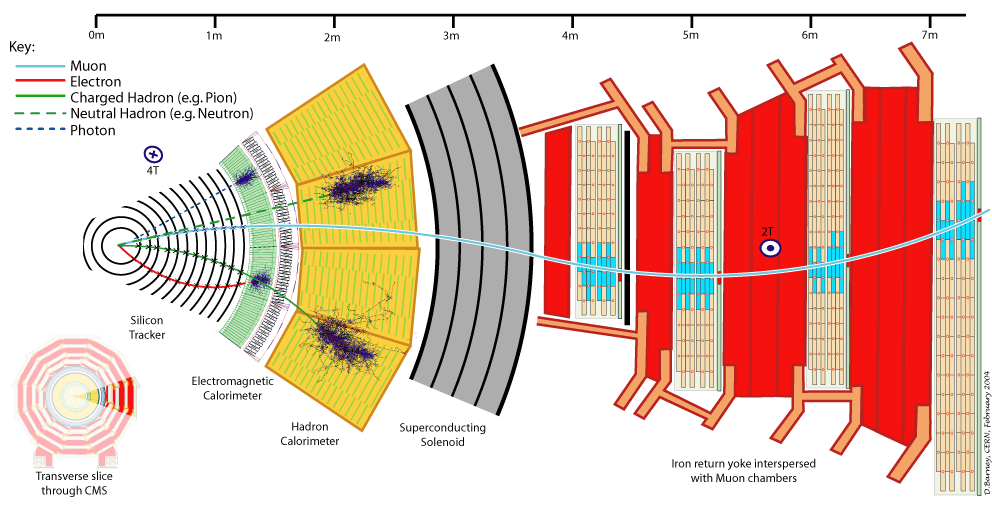
\includegraphics[width=0.99\textwidth]{plots/intro/CMS_Slice.png}
\caption{Transverse slice of the CMS detector. For each type of particle, namely muon, electron,
 photon and the neutral or charged hadron, the characteristic
signatures left in the relevant subdetectors are shown. \label{fig:cmsslice}}
\end{figure}
 
In this process, the identification of the particle type (photon, electron, muon, charged hadron, neutral hadron) plays an important role in the determination of the particle direction and energy. Photons (\eg coming from \Pgpz\ decays or from electron bremsstrahlung) are identified as ECAL energy clusters not linked to the extrapolation of any charged particle trajectory to the ECAL. Electrons (\eg coming from photon conversions in the tracker material or from \cPqb-hadron semileptonic decays) are identified as a primary charged particle track and potentially many ECAL energy clusters corresponding to this track extrapolation to the ECAL and to possible bremsstrahlung photons emitted along the way through the tracker material. Muons (\eg from \cPqb-hadron semileptonic decays) are identified as a track in the central tracker consistent with either a track or several hits in the muon system, associated with an energy deficit in the calorimeters. Charged hadrons are identified as charged particle tracks neither identified as electrons, nor as muons. Finally, neutral hadrons are identified as HCAL energy clusters not linked to any charged hadron trajectory, or as ECAL and HCAL energy excesses with respect to the expected charged hadron energy deposit. 

The energy of photons is directly obtained from the ECAL measurement, corrected for zero-suppression effects. The energy of electrons is determined from a combination of the track momentum at the main interaction vertex, the corresponding ECAL cluster energy, and the energy sum of all bremsstrahlung photons attached to the track. The energy of muons is obtained from the corresponding track momentum. The energy of charged hadrons is determined from a combination of the track momentum and the corresponding ECAL and HCAL energy, corrected for zero-suppression effects, and calibrated for the nonlinear response of the calorimeters. Finally the energy of neutral hadrons is obtained from the corresponding calibrated ECAL and HCAL energy. 

\subsection{Jet reconstruction}

For each event, hadronic jets are clustered from the particles reconstructed with the PF algorithm
 with the infrared and collinear safe
 anti-$k_\mathrm{t}$ algorithm 
operated with a size parameter $R$ of 0.5. The size parameter requires that all the jet 
particles have $\Delta R \leq 0.5$ relative to the jet momentum vector, where
 $\Delta R=\sqrt{(\Delta\phi)^2 + (\Delta\eta)^2}$ \cite{Cacciari:2008gp}. 
The jet momentum is determined as the vectorial sum of all particle momenta in this jet.
For jets originating at the event primary vertex the jet momentum is found in the simulation to be within 5\% to 10\% of the true momentum over 
the whole \pt spectrum and detector acceptance. 
When the jet origin is significantly displaced from the event primary vertex, the reduced 
charged particle efficiency results in additional underestimation of the jet momentum. 
For displaced jets originating within the volume of the CMS tracker the jet momentum is underestimated in the simulation by up to 10\%.
%Jet energy corrections are derived from the simulation, and are confirmed with in situ measurements with the energy balance of dijet and photon+jet events~\cite{CMS-PAS-JME-10-010}. The jet energy resolution amounts typically to 15\% at 10\GeV, 8\% at 100\GeV, and 4\% at 1\TeV.

